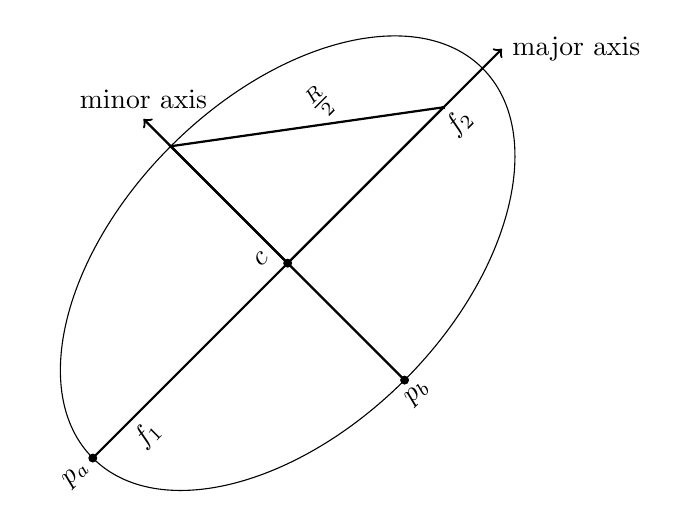
\begin{tikzpicture}[xscale=0.7, yscale=0.7][domain=0:11]
   % \draw [help axis] (-5,-3) grid (5,3);

    \begin{scope}[rotate=45]
    \draw (0,0) ellipse (5cm and 3cm);
    \node[rotate=45][below] at (-4,0) {$f_1$};
    \node[rotate=45][below] at (4,0) {$f_2$};
    \draw[fill] (-4,0) circle [radius=.5pt];
    \draw[fill] (4,0) circle [radius=.5pt];
    \draw [thick] (4,0) -- (0,0) -- (0,3) -- (4,0);
    \draw[->,thick] (-5,0)--(5.5,0) node[right]{major axis};
    \draw[->,thick] (0,-3)--(0,3.7) node[above]{minor axis};
        \node[rotate=45] [left] at (0,0.4) {$c$};
    \node [rotate=45][right] at (2.1,1.65) {$\frac{R}{2}$};
    
   
    \node [rotate=45][left] at (-5,0) {$p_a$};
    \draw[fill] (-5,0) circle [radius=2pt];
    
        \draw[fill] (0,0) circle [radius=2pt];
    
    \draw[fill] (0,-3) circle [radius=2pt];
    \node [below][rotate=45] at (0,-3) {$p_b$};
    \end{scope}

    %a^2-b^2=c^2 -> c^2=25-9=16 -> c=4
    
    %\draw[fill] (0,0) circle [radius=.5pt];
	
    %
    %\draw[fill] (5,0) circle [radius=1pt];
    %\draw[fill] (0,3) circle [radius=1pt];
    %
    

    %\node [below] at (2.1,0) {$c$};
	%\node [left] at (-0.1,1.5) {$b$};



    %\node [above] at (5,0) {$(x_0+a,y_0)$};
    %\node [above] at (-5,0) {$(x_0-a,y_0)$};
    %\node [above] at (0,3) {$(x_0,y_0+b)$};
    %
    

    
    %\draw [-] (-5,0) -- (5,0);
     %\draw [-] (0,-3) -- (0,3);
     %\draw [|-|] (0.001,-0.1) -- (4.999,-0.1);
\end{tikzpicture}